\section{联合体}
联合体初看上去很像结构体,它们的定义语法极其相似,但是它们是完全不同的事物。
\begin{lstlisting}
union ValType {
    int val_i;
    long long val_ll;
    char val_c;
    double val_d;
    long double val_ld;
};
int main() {
    cout << sizeof(ValType); //输出8或16,总之不是29或者更大的数
}
\end{lstlisting}
一个结构体会把所有成员分别存储在不同的内存区域中,所以这个类型的内存占用不能小于所有成员的总和。以第2节中定义的 \lstinline@Cuboid@ 类型为例,我们可以用这样一段代码来观察某个对象各成员的地址:
\begin{lstlisting}
    Cuboid cub;
    cout << &cub.length << endl << &cub.width << endl << &cub.height;
\end{lstlisting}
下面是一种可能的运行结果:\\\noindent\rule{\linewidth}{.2pt}\texttt{
0x7ffeea18b070\\
0x7ffeea18b074\\
0x7ffeea18b078
}\\\noindent\rule{\linewidth}{.2pt}\par
从结果中我们可以看到,\lstinline@cub@ 的三个 \lstinline@int@ 型成员分别在不同的内存空间中,\lstinline@cub.length@ 在 \lstinline@...070@ 到 \lstinline@...073@ 位置,\lstinline@cub.width@ 在 \lstinline@...074@ 到 \lstinline@...077@ 位置,\lstinline@cub.height@ 在 \lstinline@...078@ 到 \lstinline@...07b@ 位置。它们之间没有任何重叠,互不干扰。\par
但联合体不然,它会把所有成员存储到同一个内存区域中。
\begin{lstlisting}
    ValType a;
    cout << &a.val_i << endl
        << &a.val_ll << endl
        << (void*)&a.val_c << endl //记得把char*转成void*输出
        << &a.val_d << endl
        << &a.val_ld << endl;
\end{lstlisting}
下面是一种可能的运行结果:\\\noindent\rule{\linewidth}{.2pt}\texttt{
0x7ffc00a4d280\\
0x7ffc00a4d280\\
0x7ffc00a4d280\\
0x7ffc00a4d280\\
0x7ffc00a4d280
}\\\noindent\rule{\linewidth}{.2pt}
这说明联合体的所有成员都在同一个位置存着呢。\par
\subsection*{联合体如何组织内存?}
正如我们才看到的那样,联合体会把所有的成员放在同一个内存区域中。所以 \lstinline@ValType@ 的内存占用不需要达到全部成员的内存占用之和,只需要等于它们之中最大的那个就行。在这里,如果你的开发环境中 \lstinline@long double@ 类型占用8字节,那么 \lstinline@sizeof ValType@ 的结果一般就是8字节;如果你的开发环境中 \lstinline@long double@ 类型占用16字节,那么 \lstinline@sizeof ValType@ 的结果一般就是16字节。\par
既然五个成员全都占用同样的内存空间,那么它们之间势必会存在冲突。回想一下章首的图6.1——我们用不同类型去解释同一块内存空间中的内容,将会得到不同的结果。在这里也是如此。如果我们用 \lstinline@a.val_i@ 去修改这段内存中的内容,那么它将会按照 \lstinline@int@ 型对信息的组织方式来存储 \lstinline@0@/\lstinline@1@ 串。在这种情况下,输出 \lstinline@a.val_c@ 或 \lstinline@a.val_d@ 往往是看不出什么有效内容的。\par
既然这些成员之间互相有冲突,那么我们为什么还要用联合体呢?这是因为,在有些情况下,一个联合体的成员是彼此互斥的,它们不会同时出现。还是以 \lstinline@ValType@ 为例,如果用一个结构体来表达它的话,需要29或更多字节才能容纳——其中有用的信息永远不超过16字节,那么剩下的空间就浪费了。通过联合体,我们可以把这些数据都存到这8或16个字节的空间当中,只要它们不同时出现,那就不会存在冲突了。
举个现实一点的例子:像Python这样的编程语言支持动态类型,即,一个变量可以在某个时候是整型,而在之后变成字符型或浮点型。而C++是静态类型语言,一个变量的类型在它定义的时候就确定下来了,不能更改。通过联合体,我们可以在一定程度上实现动态类型的部分功能。\par
\begin{lstlisting}
struct dynamic { //自定义动态类型
    enum Types{integer,floating,string}; //枚举,用来规定可能的类型
    Types type; //type用来标记当前的类型
    union Value { //联合体,它的三个成员不会同时出现
        long long vll; //整型
        long double vld; //浮点型
        char str[16]; //字符串型
    };
    Value value; //定义Value类的对象value
};
\end{lstlisting}\par
我来解释一下这段代码:我们定义了一个 \lstinline@dynamic@ 类,这个类的对象可能以三种状态存在:整型状态,浮点型状态或字符型状态。\lstinline@type@ 是一个枚举类型,它可以用来标记这个对象当前处于何种状态。\par
而在联合体 \lstinline@Value@ 中,三个成员 \lstinline@vll@, \lstinline@vld@ 和 \lstinline@str@ 分别是整型、浮点型和字符串型。在任何时刻,这个变量只能是这三种类型之一,所以它们不会同时出现,用 \lstinline@union@ 就很合理。\par
需要读者留意的是,在 \lstinline@dynamic@ 中定义 \lstinline@Value@ 的操作不会直接引入一个什么实体。如果我们不用 \lstinline@Value value@ 这句来定义一个 \lstinline@Value@ 类的对象,那么这个内嵌的定义就没有什么存在感了。\par
\subsection*{如何使用联合体?}
那么我们就在主函数中定义一个 \lstinline@dynamic@ 类的对象,并设置它的类型和值。
\begin{lstlisting}
    dynamic number {dynamic::integer}; //integer在dynamic域中,所以用dynamic::
    number.value.vll = 15; //修改dynamic.value的vll成员,把它变成15
\end{lstlisting}
这里需要注意,\lstinline@integer@ 是 \lstinline@dynamic@ 域中的枚举项。如果我们要在域外使用,就必须用 \lstinline@dynamic::integer@。相关细节,我们留到第七章再谈。\par
在本段代码中,我们定义了一个 \lstinline@number@ 变量,并初始化它的 \lstinline@type@ 成员为 \lstinline@integer@。接下来,我们用 \lstinline@number.value.vll@ 来为 \lstinline@value.vll@ 成员赋值。一旦为 \lstinline@vll@ 赋值,这时 \lstinline@vll@ 就是活跃成员,而 \lstinline@vld@ 和 \lstinline@str@ 都是不活跃成员。试图访问不活跃成员是未定义行为,会得到不确定的结果\footnote{约等于定义了局部变量但还没有赋值/初始化就开始使用它,会得到不确定的结果。}。\par
下一刻,我们想把 \lstinline@number@ 改成浮点型。这个操作非常简单,只要为 \lstinline@vld@ 赋值,就可以把它变成活跃成员,顶掉 \lstinline@vll@。\par
\begin{lstlisting}
    number.type = dynamic::floating; //修改number的类型,标记为浮点数
    number.value.vld = number.value.vll; //vld将取代vll成为活跃成员
    cout << number.value.vld; //会输出15
\end{lstlisting}
第一行的操作就是更改一下标签,不必多说。第二行的操作却有些费解——不是说同一个联合体的不同成员不该同时出现吗?为什么我们在这里可以用 \lstinline@vll@ 给 \lstinline@vld@ 赋值还不产生问题呢?\par
其实这就是``同时''的问题了。赋值运算符不是一下子就把右操作数的值赋给左值的。赋值操作的内部过程可以分成两步:第一步是处理右操作数,把右操作数的值转移给一个临时变量\footnote{这是一个左值到右值的转换,可能还会伴随类型转换。};第二步是把这个临时变量的值转移给一左操作数,临时变量销毁。我们看,在第一步的时候 \lstinline@vll@ 是活跃成员,这时我们没有用到 \lstinline@vld@,没有问题;而在第二步的时候 \lstinline@vld@ 是活跃成员,这时我们没有用到 \lstinline@vll@,也没有问题,如图6.10所示。\par
\begin{figure}[htbp]
    \centering
    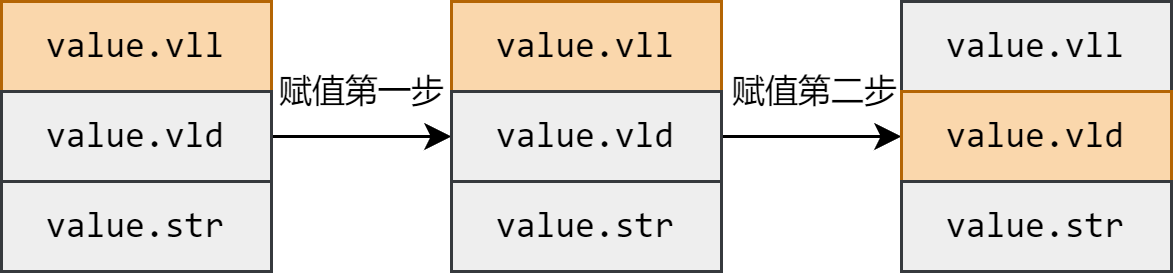
\includegraphics[width=0.8\textwidth]{../images/generalized_parts/06_process_of_assignment_to_union_300.png}
    \caption{赋值过程中,活跃成员的变化}
\end{figure}
试过了这些简单功能之后,我们可以写一些函数来实现它们。以下是一个输出函数,它根据 \lstinline@type@ 来判断要输出哪个成员。
\begin{lstlisting}
void output(const dynamic &number, ostream &out = {cout}) {
    switch (number.type) { //用switch来判断number.type的值
        case dynamic::integer: //如果是整型
            out << number.value.vll; //输出vll
            return; //直接用return返回;或者用break也行
        case dynamic::floating: //如果是浮点型
            out << number.value.vld; //输出vld
            return;
        case dynamic::string: //如果是字符串
            out << number.value.str; //输出str
            return;
    }
}
\end{lstlisting}
这个函数仍然沿袭我们的思路,以 \lstinline@cout@ 作为输出的默认参数。在函数中,我们用 \lstinline@switch@-\lstinline@case@ 结构来实现对 \lstinline@number.type@ 的判断。这个函数没有什么技术含量,读者想必很容易就能看懂。\par
\begin{lstlisting}
dynamic& assign_int(dynamic &number, long long ll) {
    number.type = dynamic::integer; //更改type
    number.value.vll = ll; //赋值给vll,现在它是活跃成员
    return number;
}
dynamic& assign_float(dynamic &number, long double ld) {
    number.type = dynamic::floating; //更改type
    number.value.vld = ld; //赋值给vld,现在它是活跃成员
    return number;
}
dynamic& assign_str(dynamic &number, const char *src) {
    number.type = dynamic::floating; //更改type
    strncpy(number.value.str, src, 16); //用strncpy为str赋值,现在它是活跃成员
    return number;
}
\end{lstlisting}
在这里,我们定义了三个函数,分别用于给 \lstinline@number@ 赋特定类型的值。至于字符串的赋值,我们提过,字符串不能直接赋值,要用 \lstinline@strcpy@ 或 \lstinline@strncpy@ 才行。这两个函数在头文件 \lstinline@cstring@ 中。\lstinline@strncpy@ 比 \lstinline@strcpy@ 更安全,它可以规定第一个操作数最多能接收的字符数量,以防字符串赋值时发生越界问题。\par
我们还可以借助联合体玩更多花样。不过相比于 \lstinline@class@/\lstinline@struct@ 来说,它的应用范围还是很窄的。接下来的章节中我们几乎不会再用 \lstinline@union@ 了,所以这里就仅为读者开拓一下眼界。想要了解关于联合体的更多用法,可以参考 \href{https://stackoverflow.com/questions/4788965/when-would-anyone-use-a-union-is-it-a-remnant-from-the-c-only-days}{When would anyone use a union? Is it a remnant from the C-only days?-Stack Overflow}。\par
